% to cite stuff use \cite{cite_key}

% Heirarchy:
%\part{part}	-1
%\chapter{chapter}	0
%\section{section}	1
%\subsection{subsection}	2
%\subsubsection{subsubsection}	3
%\paragraph{paragraph}	4
%\subparagraph{subparagraph}	5

\documentclass{article}
\usepackage{times}
\usepackage{cite}
\usepackage[autostyle]{csquotes}
\usepackage{marginnote}
\usepackage{listings}% for source code styling
\usepackage{xcolor}
\usepackage{booktabs}% For stacking in tables

% To draw a box
\usepackage{amsmath}%
\usepackage{MnSymbol}%
\usepackage{wasysym}%

% to avoid having to escape all underscores in URL's to avoid "missing $ inserted" error.
\usepackage{url}

% to include PDFs
\usepackage{pdfpages}

% For column centering in the questionnaire
\usepackage{array}
\newcolumntype{P}[1]{>{\centering\arraybackslash}p{#1}}

% Paragraph that starts on a new line.
\newcommand{\myparagraph}[1]{\paragraph{#1}\mbox{}\\}

%\textwidth = 490pt

\usepackage{graphicx}
\DeclareGraphicsExtensions{.pdf,.png,.jpg}
\graphicspath{ {./figures/} }

\setlength{\parskip}{0.6em}

\begin{document}

\title{Bringing Knowledge Through AI and SMS}
\author{Sam Heather\\
  Department of Computer Science,\\
  The University of York,\\
  \texttt{sam@heather.sh}}
\date{\today}
\maketitle
\thispagestyle{empty}

\newpage

\begin{abstract}

\marginnote{It is early days so it is normal that many things are missing from the abstract. You should keep in mind that it should include later on few sentences on method/experiment, result and conclusion.}

In remote Africa there are millions of disadvantaged and uneducated individuals, who in the vast majority do not have access to the internet the knowledge that this brings.  Outside of their immediate friends and family, individuals cannot access the information they need to further their education, or just for general interest.

In many parts of the world, the number of people without access to the internet but access to a mobile phone is significant.  This project aims to research and develop a system capable of bringing knowledge through a question and answer based interactive system, in the language natively spoken by the user, through the use of a simple Artificial Intelligence and an SMS interface.  The system will be expandable, such that it can be adjusted to handle questions on any knowledge area.

This project raises ethical issues relating to the responsibility of providing accurate information when in a position of trust, the ethics of machine translation and maintaining user privacy.
% TODO - finish abstract
\end{abstract}

\newpage
\tableofcontents
\newpage
\listoffigures
\newpage
\listoftables
\newpage

\section*{Statement of Ethics}
% TODO write this
{\bf Pretty much the most important part - write this!}
 - data protection - users information irreversibly obscured and protected in the database to protect them in case of database hack.
 - data protection - supervisor had root password to the server.
 - experiment - participants were asked to sign consent forms, these were stored with supervisor.
 - after experient, all participants were anonymised by a unique participant id, and the only mapping of these to names is the consent form, which the supervisor has
 - ethics of providing information - steps taken to try and prevent wrong info been returned

\newpage
\section*{Acknowledgement}
The author would like to acknowledge the following individuals for their contribution to this project:

\begin{itemize}
  \item SpazioDati (http://spaziodati.eu/) for providing extended access to the Dandelion Text Semantics API at no extra charge.
  \item Rackspace for providing server infrastructure.
  \item Julie Markham and Nicholas Hopper, with whom the author collaborated with on Shy, the mobile application that inspired this project.
  \item Lilian Blot, for his time and effort spent supervising and providing guidance for this project.
\end{itemize}

\newpage
\section{Introduction}

\subsection{Background of this project}

The inspiration for this project originates from a project the author undertook in September 2014 whilst attending Yacht Hack, a week-long hackathon on a Yacht in Croatia\footnote{http://toughhackers.com/yacht-hack-2014/}.  The author co-created a project called Shy to prototype a mobile application that would facilitate the immediate answering of questions that fall within certain categories using a knowledge base, simple machine learning and profiling of users based on their usage history.

One of the initial goals of Shy was to bring knowledge via m-learning\footnote{M-Learning: learning using tools available on a mobile device} as opposed to e-learning\footnote{E-Learning: learning conducted online, usually with the help of a computer}.  This is because m-learning systems are available to a much larger demographic of people, because the hardware (mobile devices, commonly phones) is becoming ever cheaper and more accessible.

A semi-functional prototype was completed for iOS, as seen in Figure~\ref{fig:shy-ios-screenshots}.  The front-end was complete; however in the backend question-answer matching was evaluated without knowledge of previous material the user had viewed.  This meant that explicitly targeted answers for a question and suggestions of questions that a given user profile might be interested in could not be made.  Up until this point, the service was restricted to working on iOS smart devices only, with poor quality question-answer matching.  In the initial project, the knowledge base was built for questions on personal health, sex, relationships and family.

\begin{figure}[htb] 
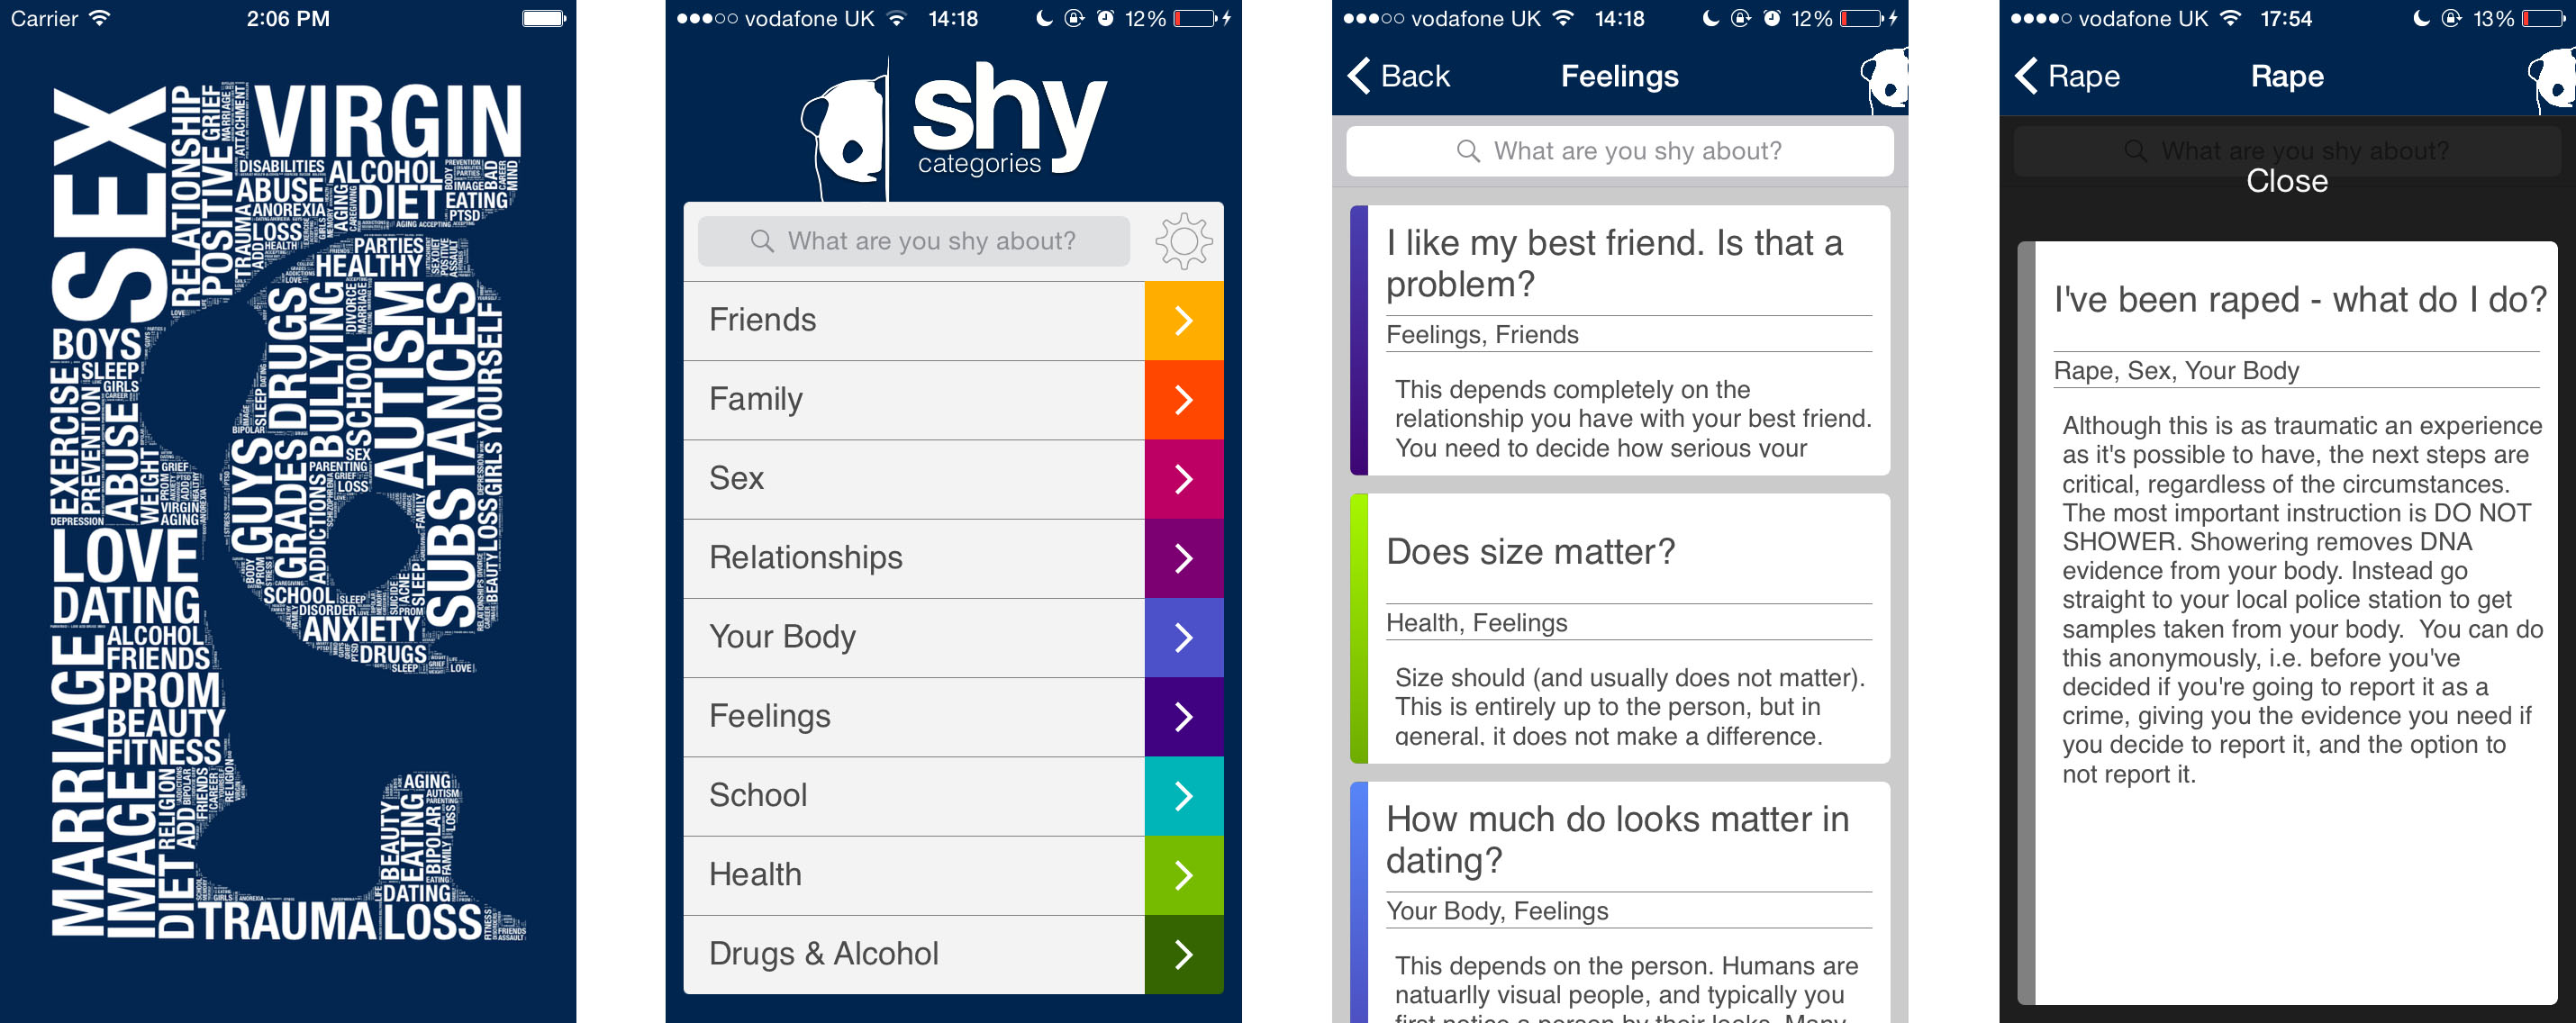
\includegraphics[width=\linewidth]{shy-screenshots}
\caption{Screenshots of Shy iOS App}
\label{fig:shy-ios-screenshots}
\end{figure}

\subsection{Motivation for this project}
Access to knowledge is a critical part of modern life.  It's also a Human Right, under Article 27 of the Universal Declaration of Human Rights~\cite{community1948universal}.  As members of a developed country, we have the facility to retrieve information and instantly communicate with each other using our smart phones, and commonly do it up to 200 times a day~\cite{falaki} which is a facility that hundreds of millions of individuals in developing countries live without.  This project aims to investigate the technical and ethical challenges behind this and to create a technology to give more people access to knowledge, and thus their human rights.

The project involves the use of a number of systems, including machine translation, an SMS input/output system and a system to build a profile on a user in order to facilitate high-quality targeted question-answer matching.  The system will also feature machine learning so that as time progresses, the quality of the answers it returns increases.  The use of these systems in one application along with complex ethics and privacy issues create an interesting project that draws together many technologies and discussions in a way that can be used as a basis for further research in the future.

\subsection{Aims of this project}

The first goal of this project is to assess and address the ethical issues that arise from the software that will be created.  These include the responsibility that the software and its developer has because of its position of trust to provide accurate information and to protect the privacy of its users by storing only necessary information, among others.  This project will do this by researching ethical issues relating to the technologies that the project will use, for example machine translation and user information storage.  This will then be used to feed the design process of the software and to specify the expected use-case of it.  Finally, the resulting software will be evaluated through experimentation, with volunteers asking the software a set of questions within a topic area, in a non-English language, and evaluate the relevance of answers returned.

Initially, the goal for this dissertation was to focus on questions relating to personal health, sex, relationships and family, which was as a direct result of the focus of 'Shy'.  Although a health and diseases database was located in the early stages of the project (Diseases Database, www.diseasesdatabase.com), it was targeted at professional uses for the data and came with a significant licence fee, as well as complex documentation that the provider customised specifically for each use-case.  An attempt was made to acquire a free academic research licence via email but this was unsuccessful.  Additionally, as the project progressed in the early stages it became clear that the author's original two-page document discussing ethical considerations with the project did not cover all possible situations.  Indeed, the Author and Supervisor\marginnote{Lilian: Should I avoid mentioning 'author' and 'supervisor' here? I want to communicate that there was effort in this. Should I reword to 'significant effort was .......'} were still discovering further significant ethical issues as far as eight weeks into the project, which would have required a complex ethics panel review, critically delaying this project.  Two example ethical issues that occurred were:

\begin{itemize}
  \item Any application has that dispenses health related information that a user might act upon in a life changing manner has to respond with correct information, since an incorrect response could lead to a user taking an action which leads to them harming themselves.
  \item Privacy is critical since the questions been asked are personal.  This could not be absolutely guaranteed, since a third-party service had to be used to send SMSs and, although unlikely, it was possible that this service could build profiles on users and identify them.
\end{itemize}

As a result of the above issues with locating a reputable knowledge base and the complex ethical issues, a decision was made in early December 2014 to switch the target topic for questions to Geography and to use Wikipedia as a datasource, since it is openly available, well populated and multiple methods exist for extracting information from it.  In future work, it should be possible to extend this project to work with medical questions, if a high quality data-source is located and a solution to the ethical issues is found. A full discussion of possible future work is included in section \ref{sec:extending}.

\subsection{Structure of this report}
This report starts with a literature review in chapter~\ref{sec:literatureReview} where existing software, tools and services of a similar type to those that will be used in this project are presented, along with research into the ethical issues of the creation and use of the software under development. Comparisons between different software development life-cycles are also described and discussed.

Chapter~\ref{sec:method} describes the method that will be taken to develop the software and service.  This covers the software development life-cycle that will be followed, and sets out a plan for when development will take place.  Requirements will also be identified, described and categorised  as either functional or non-functional.  A method of evaluating the success of the software will also be discussed and chosen.

The design of the software, driven from information collected from the requirements, will be set out in Chapter~\ref{sec:design}.  The individual components that make up the technology will be described and discussed, followed by a set of annotated diagrams showing how these modules will interface with each other to build a complete system.  Finally, this section will include a description of the platform, language and other tools that will be used.

Chapter~\ref{sec:implementation} contains details about the implementation of the software.  This includes information on the tools that will be used to create components such as the SMS interface and question-answer matching system.

Results from the evaluation of the system will be presented in Chapter~\ref{sec:results}.  A discussion of these results and their implication on this project is then presented to the reader in Chapter~\ref{sec:discussion}.

Chapter~\ref{sec:evaluation} contains an evaluation of the software produced and the process taken to complete it.  Comparisons will be made to the success criteria, set out for the project in section \ref{sec:evaluatingSuccess}.

Thoughts on potential future research that builds on the work produced in this project are then displayed in chapter~\ref{sec:extending}.

Finally, the main achievements of this project are concluded in chapter~\ref{sec:conclusion} with closing thoughts.


% Lilian: This section should be expended, especially mentioning the consequences of such assumptions. Why do you make those assumption (e.g. time constraint, little or no consequences, ...). What limitation this may cause to your findings.  Shows a mastery of the field.
\subsection{Assumptions Within This Project}
This project will make the assumption that users of this service have basic literacy skills in \marginnote{Lilian: I no longer have language support, and you said to keep research in about it. Should I remove it from introduction / abstract etc?}a language supported by the project.  Although this is not a correct assumption world-wide, expanding the remit of this project to include a 'graphical' user interface that works over SMS would scale this project outside of the practical limitations of this project.

The main use-case for this project is going to be parts of the world with limited internet access.  Although these exist all over the world, the African continent is typical of this problem so I will focus my research in demonstrating a need for this tool there.

{\color{red} extend this}

\newpage

\section{Literature Review}
\label{sec:literatureReview}

{\bf The point of this is to show that I 'own' the material and subject (competence).  Show different points of view, choose a side, express a view on which I prefer and if I agree, critique.  Have objective goals.}

% TODO expand introduction to explain why sms, then look at related work in next section.  compare to smart phones loosely.
A significant amount of work has previously been undertaken in the area of making knowledge quickly accessible to us in the form of questions and answers.  To take one example, imagine that an individual needs to find the population of London as quickly as possible.  The initial step would be to search for information.  In the connected world, this is easy: a simple Google search returns the answers without even having to click through to any resources, as shown in Figure \ref{fig:googleInstant}.

\begin{figure}[htb] 
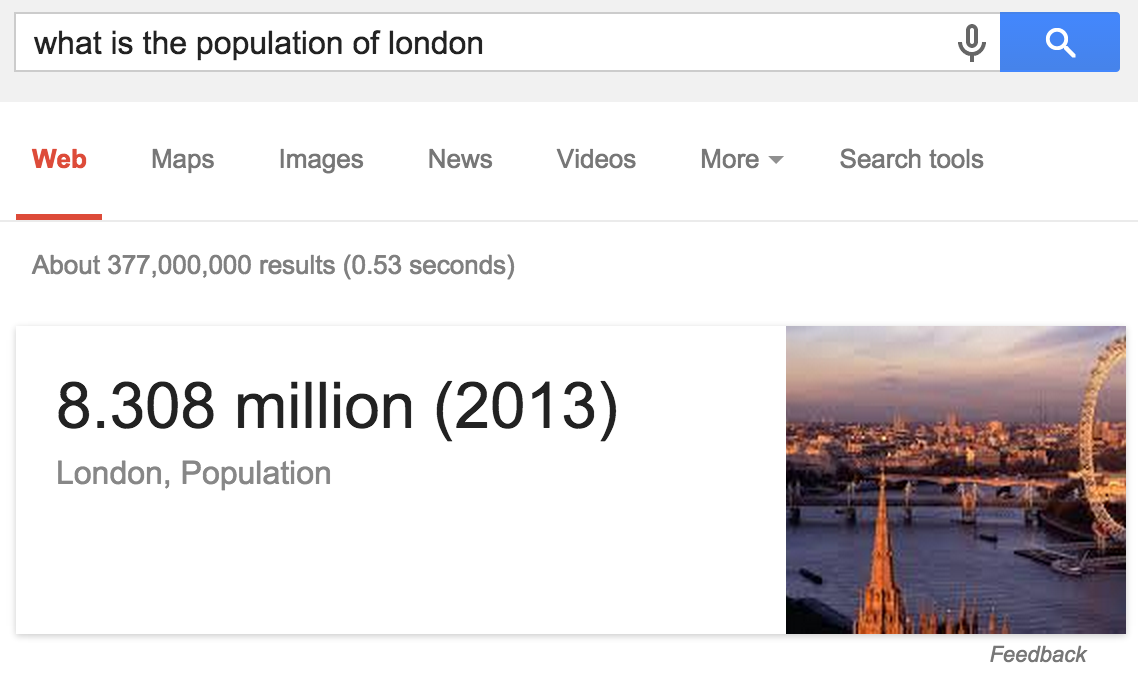
\includegraphics[width=\linewidth]{googleInstant}
\caption{Google Now information box.  Screenshot taken on 3rd February 2015.}
\label{fig:googleInstant}
\end{figure}

This is easy to do in the developed world where up to 75\% of the population are connected to the internet~\cite{ITU_Cell_Usage_2013}, with the population of elderly people been largely responsible for the remaining 25\%~\cite{Gov_Internet_Usage_UK_2014}.  This contrasts strongly with the situation in the African continent, where in 2013, internet usage had only reached 16\%~\cite{ITU_Cell_Usage_2013}, a figure largely inflated by South Africa where 5\% of the African population generate 2/3 of internet traffic from the African Continent~\cite{ITU_Cell_Usage_2013}.

% But there are other communication methods which are proven to work
\subsection{Previous work using SMS}
Although the above suggests that the African continent is majoritively disconnected, this is not the case.  Because of restrictions in the electricity available, the ways in which a non-smart phone \marginnote{\color{red}cite that these are lower power consumption, or assume?  Emma: Isn't necessary but would be helpful; leave it up to whether you need to fill out your word count or cut down.} can be used in Africa have far surpassed those in the developed world~\cite{Fox:2011:Online}, in part due to the low power consumption of a non-smart mobile phone.  Interesting examples of SMS use in Africa include an automated service which sends an SMS to HIV/AIDS sufferers to remind them to take their medication, and a system for farmers that gives them the current market prices for goods, saving them from making regular long-distance trips to the market or relying on out-of-date information from a weekly radio broadcast~\cite{Aker_Mobile_Phones_2010}.

Interactive systems have also been developed to operate over SMS.  One successful example is mobile money platforms.  These allow for users from any background to pay and be paid for goods and to transfer money across long distances at negligible cost~\cite{Aker_Mobile_Phones_2010}.  One of the most highly adopted services is M-Pesa, which in Kenya alone was responsible for \textsterling5.7 Billion in transfers in 2012 \footnote{Data from Safaricom, M-Pesa operator in Kenya - actual value 817,085,000,000 Kenyan Shillings, converted to GBP on 1st November 2014 at rate of approximately 0.007.}.  M-Pesa gives users a balance linked to a national ID number from which they can pay for goods by sending an SMS with a cashier (recipient) number or pay outstanding bills in a similar way.  Non-subscribers can also use the system by depositing money with a M-Pesa cashier in exchange for an access code, which can be sent via SMS to a contact who can subsequently redeem it with their local cashier~\cite{Aker_Mobile_Phones_2010}.

This difference in standard use of mobile phones is demonstrated in the International Telecommunications Union's 2013 report~\cite{ITU_Cell_Usage_2013}, which shows that in Europe, for 790 million mobile subscriptions, 53\% of subscribers have mobile internet access (422 million), compared to 17\% in Africa (93 million have mobile broadband, out of 545 mobile subscribers).  This is due to the prohibitively high cost of accessing data services, regardless of the hardware that the user has.  In 2012 in Europe, 500 MB of data per month for 12 months cost 1.2\% of the average Gross National Income Per Capita (GNI pc).  In Africa, the average price was 30x this, at 36.2\% of an individuals GNI pc~\cite{ITU_Information_Society_2013}.

% No research has been undertaken investigating whether bringing knowledge through this method is viable option.

\subsection{Ethical Issues}
This project raises a number of ethical issues related to translation accuracy, providing information to people in an ethically acceptable way (with a focus on information accuracy) and maintaining user privacy.

\subsubsection{Ethics of Providing Information}
One significant issue for this project stems from providing information that may affect an individual or lead them to take a harmful action.

% TODO Finish Ethics of Providing Informatio

{\bf In a similar way to that which a teacher has a responsibility to teach accurate information to a pupil due to their position of trust, any service relied upon by a user must equally provide accurate information.  The result of not doing this could be providing inaccurate information that leads to a user carrying out an action that causes harm}.

% TODO Reword last two sentences.  This is something important and obvious - perhaps simple analogy is not necessary.  Perhaps give a generalised example.

% Lilian: You may want to look toward news paper (online/printed) to look at current/past issues that led to a law suit/inquiry and subsequent verdict/laws that may have been changed.

% Lilian: You should provide both point of view so do use this material, then you will have to critic both point of views. 
{\bf this needs to be waaaayyyyy expanded, but I struggled to find information that was useful.  There's lots on remote education, and on basic ethics of teaching, but I struggled to find anything specifically relating to ethics of ensuring information you provide is correct}.

\marginnote{teachers code of conduct, wikipedia ethics to provide infomration that contributos believe to be correct. doctors and gp's provide to the best of their knowledge}

\subsubsection{Ethics of Translation}
A significant part of this project is represented by the support of multiple languages.  It is clear that translation on demand, at scale, needs to be automated by some kind of machine or algorithmic translation.

This project involves two blocks of translation.  These are:
\begin{itemize}
  \item The translation of the user's input into the language of the system (English)
  \item The translation of the answer to a user's question from the system language to their local language.
\end{itemize}
The latter of these raises some issues that do not apply to the former. To understand these issues it is first necessary to understand the two categories of machine translation.

Rule-based machine translation effectively treats human language in a similar style to programming languages.  Formal grammars and lexicons are used to represent words that exist in either the source or target language, structures representing the translation of individual words or groups of words.  Map structures contain mappings between individual or groups of words to their translated counterparts, sometimes with multiple results (a 1-to-many map), from which rules decide which is selected.  Maps and rule sets are created by trained computational linguists~\cite{kenny2011ethics}.

More commonly, Statistical Machine Translation (SMT) is used, for example, by Google and Microsoft in their translation products~\cite{kenny2011ethics, Google_Translate_Research}.  SMT learns mappings between strings of words of potentially unequal lengths from pre-existing original texts and their trusted human translations.  The accuracy and breadth of language support for translation increases as more source material is analysed by the system, as potentially erroneous or low quality translations can be identified and flagged.  SMT is also dependent on the quality of the human translation on the input material~\cite{kenny2011ethics}.

A significant issue that is present in statistical machine learning systems comes from the knowledge we assume an individual has and derives from a word; in this project, this affects the translation of the answers returned to a user.  In human translation this is solved by the translator's knowledge of the difference in material culture, allowing them to append necessary information to the resulting translation that the recipient might find useful.  In statistical machine learning, cultural awareness of material knowledge is a separate problem on its own.  {\bf formal reference to this, probably again from Kenny, but should be able to find better}.  To take one example from Melby (2006):

\blockquote{"when translating a French menu, a human translator might stop to think that an English speaker in France would appreciate being told that a steak tartare is served entirely raw, even if this information is not contained in the original text (because French people might be assumed to know this already). Such a translator would be aware of differences in material culture, and would be able to empathise with the English speaker who might choose to avoid the dish, given more information"~\cite{melby2006can, kenny2011ethics}}
\marginnote{Lilian: quote taken from~\cite{kenny2011ethics}, but quote is interpreted from~\cite{melby2006can} - so I think referencing both is correct, but for this reason rather than last reason we discussed?}

This issue is a result of the translation engine not being capable of taking and using a complete representation of the expected cultural differences between those who speak the input language and those who speak the output language~\cite{melby2006can}. This does not apply to the first block of translation within the application where a user's input is translated into the language of the system, since the application will only need to parse text to identify geographical entities and the property been queried, making context unnecessary.

{\bf below should really be expanded and be in the discussion.  Explain the decision to keep translated answers in the database, which are pre-approved, to ensure no cultural misunderstandings.}

The potential uses of this system include distributing information that may be used by individuals making important decisions, regardless of whether that is within this project or in further work based off of this project, as cultural confusion such as this could have potentially catastrophic effects.

\subsubsection{User Privacy and Data Protection}
\label{subsubsec:userPrivacyAndDataProtection}
This project uses a simple Artificial Intelligence (AI) to keep a record of information that has already been returned to a user, to attempt to save sending repetitive information (saving the cost of additional SMS).  This raises another ethical issue though of privacy.  The material that a user has researched is likely to be sensitive; such is the nature of health related questions\marginnote{Lilian: Need to re-write this for new question subject, or can leave as a mark of the old subject topic?}.  This means that the information on a user has to be kept securely, in a way that an individual user can not be identified.

One way of doing this is using a technology called hashing.  Hashing is the technique of taking data as an input and generating an output value (called a 'hash') that is unique to an input.  Hash functions are ideally one way functions where given a piece of input data X, the output hash will always be a constant value Y, whenever and however the hashing algorithm is executed.  This allows a user's identifying information such as their phone number to be obscured, in such a way that the mobile number can not be recovered from the database.  When a question is received, the phone number (represented by variable X in the above example) can be hashed and the data for this number looked up from the database without the database application ever being aware of the phone number of the user.  In the example in Figure~\ref{fig:hashPhoneNumber}, a phone number (X) is used as input to an imaginary hashing function and the output hash (Y) is shown on the right hand side.  As just described, this number can then be used as the key for the user information database, shown in Table~\ref{table:hashDatabase} to retrieve the information needed for the AI.

{\bf reference the above from security engineering ross anderson, chapter 10 and 21?}

\begin{figure}[htb]
    \centering
    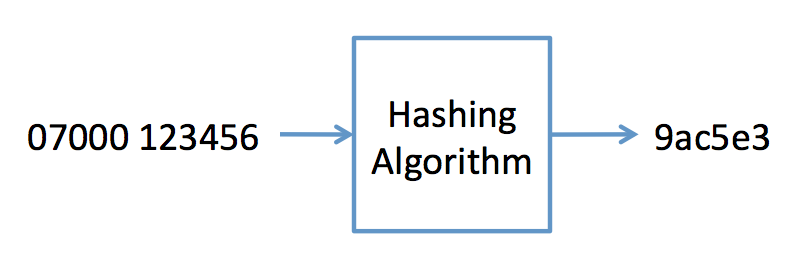
\includegraphics[width=200pt]{hashPhoneNumber}
    \caption{Hashing a phone number using an arbitrary hashing algorithm}
    \label{fig:hashPhoneNumber}
\end{figure}

\begin{table}
\begin{center}
    \begin{tabular}{| l | l |}
    \hline
    userId & userData \\ \hline
    8f64B2 & \{‘previousQuestions’:[13,301,170,577]\} \\ \hline
    9ac5e3 & \{‘previousQuestions’:[441,56]\} \\ \hline
    f9dd7e & \{‘previousQuestions’:[301,623,89,280,364,621,209]\} \\
    \hline
    \end{tabular}
    \caption{Example of software database: hashed phone numbers paired with a list of previous returned answer IDs. }
    \label{table:hashDatabase}
\end{center}
\end{table}

In practise it is possible for the output of a hashing algorithm not to be unique to a particular input.  This is known as the collision resistance property of a hashing algorithm and formally is the property of a hashing algorithm that determines the probability of the same output hash for two distinct random inputs~\cite{mitCryptographyMd5}.  It occurs because the range of possible input values is much larger than the range of output hashes, and because all valid inputs must map to an output there is repetition in outputs~\cite{mitCryptographyMd5}.  This property of hashing algorithms can be a security risk for some use-cases, where hashes are used to verify that data has not changed since been hashed.  In this case, a third-party may be attempting to generate alternative, malicious data with the same hash as some pre-existing data, to swap them undetected~\cite{securityEngineeringHashingAnderson}.  In the use-case of this project there is no security risk since hashes are only used to anonymise phone numbers; however a high collision resistance is necessary to ensure that two users of the system with distinct phone numbers don't get mapped to the same row in the database, resulting in poor quality question-answer matching or in the extreme worst case, privacy issues originating from returning to one user answers that are targeted to another.

Irreversibility is a necessary property of the hashing algorithm chosen for this project.  This ensures that the key used in the database cannot be used to retrieve the phone number of the user, thus protecting their identity.  Commonly used hashing algorithm families, such as the MD family (e.g. MD5) and SHA family are all designed to be one-way~\cite{schneierCryptanalysisMD5SHA}\footnote{Bruce Schneier is a fellow at Harvard's Berkman center for internet and society.  He has been posting regularly for his newsletter and then blog since 1998 (over 16 years) and has published material related to this field throughout this time.  He has been involved in the creation of other cryptographic algorithms, such as the Skein hashing algorithm, blowfish block cipher, so may have a vested interest in discrediting other algorithms such as MD5 and SHA.  However, the essay cited above is written as a result of the Crypto 2004 Conference in California, where the algorithm that Schneier suggests should be used at the end is not one that he has involvement in.  For these reasons, I believe this source is reliable.}\marginnote{Lilian: Dump the whole footnote?}.  

Although hashing algorithms are computationally one-way, they can suffer from another type of vulnerability affecting the security of the original input data.  When hashes are used for short strings of information (passwords, for example), a simple way to try and retrieve the original data is to compute a dictionary of the hashes of lots of common passwords, from which matches can be found.  This idea has been extended to produce Precomputed Hash Chains and subsequently Rainbow Tables.  These are highly efficient data structures that consist of chains of processed input messages and their hashes with a reduce function to reach the next item in the chain, allowing original input data to be looked-up from its hash.  Both Precomputed Hash Chains and Rainbow Tables tend to be Terabytes in size, and as such they only exist in a significant form for the most commonly used hash functions (including MD5 and SHA)~\cite{Teat:2011:SCH:2016039.2016072}.  Within this project, this raises privacy implications, as hashes within the database would be 'convertible' to phone numbers.

In password authentication systems, this can be solved by the use of a technique called Salting~\cite{hashingPasswordsInfoSec}.  Salting is where a 'salt' - a piece of additional unique data - is added to each piece of input data before hashing, and then this salt is prepended to the output hash.  This nullifies the use of Precomputed Hash Chains and subsequently Rainbow Tables~\cite{hashingPasswordsInfoSec}. When checking if a plaintext password is equal to the hashed and salted representation, the salt from the stored hash is added to the plaintext password, the hashing algorithm applied and then the output compared to the stored obscured password. However, in this application this would prevent efficient lookup of users from phone numbers in the application, as the application would have to compare an input phone number against every user object in the database, which is computationally expensive and slow since a salted hash has to be computed for potentially every user record~\cite{hashingPasswordsInfoSec}.  

As such, it has been decided that the best way of protecting a user's phone number in the event of a database hack without significantly degrading performance is to salt phone numbers with a constant, large and complex salt. This means that a rainbow table would have to be specifically computed specifically for this application and would be extremely large in size.

\subsection{Software Design Life Cycles}
There are many software development life cycles that a developer or company has available to choose from.  Four common ones include the Waterfall Model~\cite{royce1970managing-FirstDescriptionOfWaterFallModelNotByName}, Iterative Model~\cite{briefHistoryOfIncrementalAndIterativeSoftwareDevelopment}\footnote{Iterative development came together from many concepts dating back to 1957.  There was no single paper that initially presented the entire concept, but this paper gives a summary of how the various concepts came together into the current Iterative Development model.}, Spiral Model~\cite{spiralModelSoftwareDevelopment} and the Agile Development Model~\cite{beck2001agile}\footnote{The Agile Manifesto brought together a group of Agile Methods which had been in use since the mid-1990's into a single concept, that of Agile Development.}.\marginnote{Lilian: Do I need to reference that these are common?} In order to choose which life cycle suits this project best, research into all four has been carried out.

line space

line space

line space

% TODO remove the above line space

\marginnote{Lilian: remove these two footnotes? Not always necessary to reference the original}

\subsubsection{The Waterfall Model}
The waterfall model consists of 5 phases of work, where each leads directly into the next.  It is a plan driven development model, which means that all process activities such as the implementation of the project must be planned and scheduled before work on them begins~\cite{sommervilleSoftwareEngineering}.  The five layers are shown in Figure \ref{fig:waterfallModel} and described below:
\begin{enumerate}
  \item {\bf Requirements}.  In this stage, both user and system requirements for the project are determined after examining the business goals for the project.  These form the system specification.
  \item {\bf Design}.  Here, a plan for the software development is created.  The overall architecture for the software is created, the external libraries to be used are chosen and the interaction between different modules is modelled.
  \item {\bf Implementation}.  In this stage, the software is implemented to match the design and architecture set out in the Design phase.  Unit tests are written to ensure that each module matches its specification.
  \item {\bf Testing}.  In this section the system is tested as a whole to check for any bugs that might not be picked up when testing individual modules in isolation.  The software is then delivered.
  \item {\bf Maintenance}.  Finally, the software is deployed and maintained.  This includes making changes to the requirements and subsequently the software implementation as the business goals change. ~\cite{sommervilleSoftwareEngineering}
\end{enumerate}

\begin{figure}[htb] 
\centering
    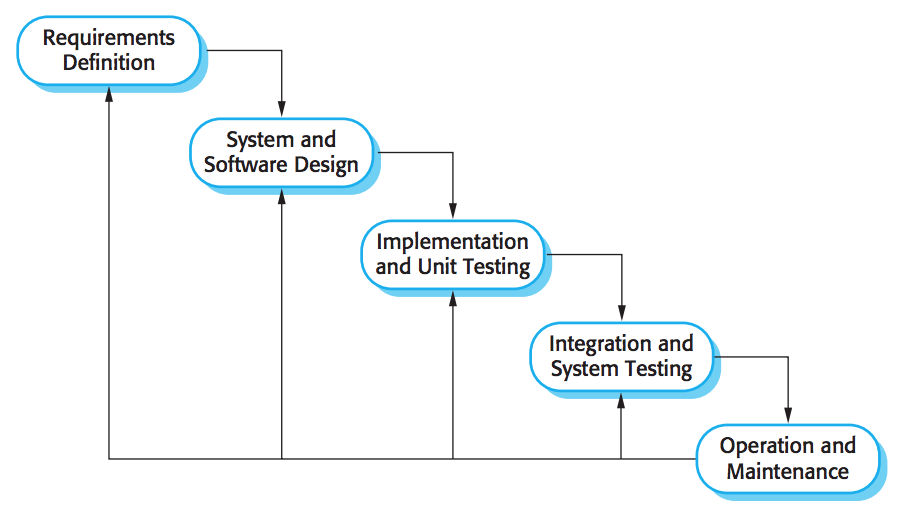
\includegraphics[width=0.8\linewidth]{waterfallModel}
\caption{Waterfall Development Model~\cite{sommervilleSoftwareEngineering}}
\label{fig:waterfallModel}
\end{figure}

A key advantage of the Waterfall Model is its simplicity: it is easy to understand and to use, saving time at the start of the project that would otherwise have been spent on learning and preparing to use a more complex model. The main disadvantage of the waterfall model is that once development has moved from one stage to another it cannot go back because the model is fixed and progresses in one direction only, until the maintenance step.

\subsubsection{The Iterative Model}
Iterative development is the practise of splitting the overall development of a project into multiple independent and distinct blocks.  A block contains a sequence of tasks which are essentially a mini life cycle, such that each iteration can really be thought of as its own project.  Each iteration tends to focus on a specific set of features such that when the iteration is complete the overall project is stable and the modules developed to date can be tested as a whole system~\cite{differenceBetweenLifeCycleModels}.

There are a multiple variations of the iterative development method. Two of these are Timeboxed Iterative Development where all iterations have a fixed duration, and Client-driven Iterative Development where each iteration contains the features that the client considers have the highest business value~\cite{larman2004agile}.

A common variation is based on the waterfall model as shown in Figure \ref{fig:iterativeDevelopment}.  The first three tasks in the cycle represent the first four stages in the waterfall model (Requirements, Design, Implementation and Testing), at which point there is the option to either evaluate progress so far and start another iteration, or to deploy the software and end development.  One significant difference between this and the waterfall model is that maintenance is not represented.

A key advantage of the Iterative Model is that it allows for the user to revise their requirements as they progress, making it dynamic and flexible which is ideal for small development teams.  This is also its disadvantage, in that the lack of fixed structure can be a weakness unless the project is planned well.

\begin{figure}[htb] 
\centering
    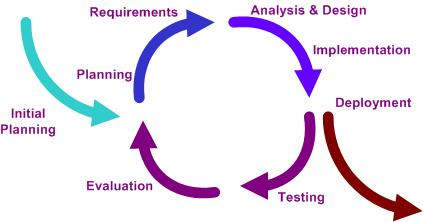
\includegraphics[width=0.8\linewidth]{iterativeDevelopment}
\caption{Iterative Development Method}
\small source: \url{https://commons.wikimedia.org/wiki/File:Iterative_development_model_V2.jpg}
\label{fig:iterativeDevelopment}
\end{figure}

\subsubsection{Boehm's Spiral Model}
The Spiral Model~\cite{spiralModelSoftwareDevelopment} was originally developed as a result of the adjustments that were commonly made to the waterfall model in large government projects.  The Spiral Model is a general model and can be used as a generator for other more specific models, given the parameters for a project such as its risks~\cite{boehm2000spiral}.  Models such as the waterfall model are specialisations of the spiral model~\cite{boehm2000spiral}.

Each loop represents a stage of the software development, from planning on the inside loop to system testing and verification on the outside, as shown in Figure \ref{fig:spiralModel}.
\marginnote{give better explanation}
% todo give better explanation

\begin{figure}[htb] 
\centering
    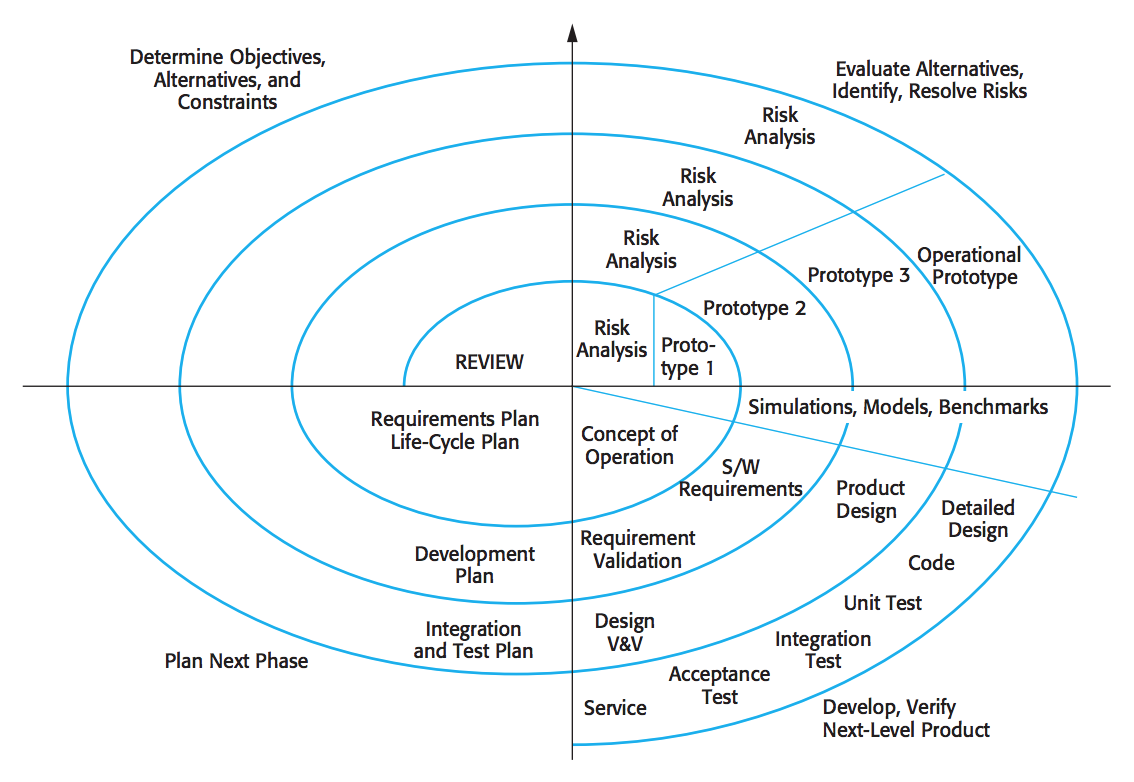
\includegraphics[width=0.8\linewidth]{spiralModel}
\caption{Boehm's Spiral Model~\cite{sommervilleSoftwareEngineering}}
\label{fig:spiralModel}
\end{figure}

A key advantage of the Spiral Model is the level of detail it models.  The stage of a sub-task within the entire development process is represented by the distance from the origin and each loop is split into small, well described sections.  The main disadvantage is that the planning and use of the model is largely driven by the results of complex risk analysis on the sub-tasks~\cite{sommervilleSoftwareEngineering}.  Although this makes it favourable to large organisations, it has the opposite effect for smaller projects.

\subsubsection{Agile Development}
Agile Development essentially represents a group of development techniques targeted towards either the development of a small to medium sized product for sale or the development of a custom system within an organisation, where the customer has a high degree of involvement, for example 'Extreme Programming'~\cite{sommervilleSoftwareEngineering}.

Agile development is highly targeted towards teams with components such as Pair Programming, Collective Ownership, regular meetings and employee health (avoiding overtime) playing an integral part in the model~\cite{sommervilleSoftwareEngineering}.

\subsubsection{Development Life Cycle Summary}
\label{sec:developmentLifeCycleSummary}
Iterative development has been chosen as the model that this project will use, based on the following factors:
\begin{enumerate}
  \item Boehm's Spiral Model and Agile Development are both targeted towards development teams.  A significant part of these models relates to team interaction, so they are not appropriate to this project.
  \item The Waterfall Model is rigid and inflexible.  It does not allow for the changes to the requirements and implementation that might be proposed after evaluating the quality of the first implementation.
  \item The Iterative development model can be implemented effectively by a single developer, and supports the adjustment of requirements and implementation in each iteration of the cycle.
\end{enumerate}


\newpage
\section{Method and Requirements}
\label{sec:method}

\subsection{Plan for Software Development}
%TODO start writing this!
The Iterative Development Model was selected in Section \ref{sec:developmentLifeCycleSummary}.  Therefore, the development of this service will follow the principles set forth in this process.

\subsection{Requirements}
\subsubsection{Use Cases / User Goals}
Two personas were created to represent individuals who may have a need for the work resulting from this project, which can be seen in Appendix A in Section \ref{sec:appendixPersonas}. These are Nanjala, who is from Uganda, and Cedric, who is from Switzerland, and it is from these that user goals are extracted. These describe what a general user aims to achieve with this service.
\begin{enumerate}
  \item Nanjala wants to be able to read general information on any given topic.
  \item Cedric wants to be able to retrieve facts from direct questions.
  \item Both Nanjala and Cedric want to be able to achieve their goals entirely via SMS.
  \item Cedric needs a simple and efficient user interface that allows him to retrieve facts quickly. 
  \item Cedric wants to be able to feedback into the system when he finds an answer particularly useful or unhelpful. 
  \item Nanjala wants to be able to show the service to her friends without explaining how to use it every time.
  \item Cedric wants the system to protect his privacy, obscuring his identity.
  \item Nanjala wants to be able to ask questions as she would ask a friend without having to learn a syntax.
\end{enumerate}

\subsubsection{User Requirements}
\label{subsubsec:userRequirements}
User goals are distilled into formal user requirements.  Each user requirement corresponds directly to the correspondingly numbered user goal.
\begin{enumerate}
  \item Users must be able to request general or descriptive information on a geographical entity.
  \item Users must be able to ask questions requesting a fact or statistic about an entity and get the answer or number they are looking for.
  \item Users must be able to interact with the system over SMS.
  \item Users must be able to make their queries and get responses quickly.
  \item Users must be able to feedback to the system when an answer is of noticeably low or high quality so the system can learn and improve.
  \item Users must be able to learn how to use the system themselves and this learning process should be quick.
  \item Users must be comfortable that their privacy is been protected whilst using the service.
  \item \label{requirement:userReqNaturalLanguage} Users must be able to interact with the system using natural language.
\end{enumerate}

\subsubsection{System Requirements - Functional}
\label{subsubsec:systemRequirementsFunctional}

System requirements are derived from the capabilities that the software needs to have to be able to support the user requirements. To support the user requirements in section \ref{subsubsec:userRequirements}, the application system must fulfil the following system requirements.

\begin{enumerate}
  \item \label{requirement:sysReqNaturalLanguage} The system will be capable of processing queries in natural language form.
  \item The system will receive queries via SMS, process them and then respond via SMS.
  \item The system shall use a datasource that contains both facts and descriptive text on geographical entities to answer queries.
  \item The system must be able to parse queries to identify the entity that is being asked about and the specific parameter of that entity that should be returned as the answer to the user's query.
  \item As well as giving direct facts and statistics, the system should be able to give general descriptive information on an entity.
  \item The system must be able to match words of similar meaning to the parameters in the data source.  For example, the word 'long' must be matched to the parameter 'length'.
  \item The system must learn from user feedback when answers that are returned are of high or low quality an apply this knowledge to future queries.
  \item The system must be self-explanatory, with the facility to offer instructions to a user.
  \item The system must use user state so that it can accept queries that are dependent on past questions, for example a query asking for more information or feedback on the quality of a past question.
  \item \label{requirement:easyToImplement} The system must be easy to implement and flexible, to accommodate future projects that make use of adaptations of this project.
  \item The system must obscure a user's phone number in the database.
\end{enumerate}

\subsubsection{System Requirements - Non-Functional}
\label{subsubsec:systemRequirementsNonFunctional}
Non-functional requirements are listed in table \ref{table:nonFunctionalRequirementsFitCrit} and are accompanied by a Fit Criterion, which will be used to identify whether a requirement has been met successfully.

\begin{table}
\begin{center}
    \begin{tabular}{| p{6.0cm} | p{6.0cm} |}
    \hline
    Non-Functional Requirement & Fit Criterion \\ \hline
    The system behind the SMS gateway must respond in a timely manner.  & From an SMS been received, a response must be sent within 20 seconds.  SMS transmission times on the cellular network and gateway are out of the control of this project, so are not accounted for. \\ \hline
    The answers returned must be of high quality.  & In testing, the system returns the correct information for at least 90\% of queries initially (before learning starts) if an answer is returned at all. \\ \hline
    Answers that are consistently rated poorly are are less likely to be returned. & In testing, after receiving a small number of negative ratings for an answer, a different answer is returned. \\ \hline
    Instructions to use the service should be clear and concise, with no ambiguity.  & In testing, having explained the purpose of the system, a user should be able to use the system with just the help information, without needing to ask for assistance. \\ \hline  
    The system should accept and be able to process questions in natural human language as opposed to a delimited message. & In testing, a user should be able to use the system for general questions without having had a syntax explained to them. \\ \hline
    \end{tabular}
    \caption{List of non-functional requirements and their Fit Criteria.}
    \label{table:nonFunctionalRequirementsFitCrit}
\end{center}
\end{table}

\subsection{Data Sources}
A number of possible datasources were identified from which data could be drawn from for this project.  These were all based off of Wikipedia (a large, linked source of knowledge), and include the Wikipedia API and various representations of the DBPedia Ontology.  In this section, both will be discussed and a decision will be made with regard to which ones will be used.

\subsubsection{Wikipedia API}
The Wikipedia API is a standard MediaWiki API and allows applications to query a page or resource for various parameters from a page, including the page contents, infobox parameters, citation list and links to other articles in various flat or multi-layered data structures~\cite{mediaWikiAPI}.  Interactions are made via a HTTP GET request to a URL containing the parameters, and responses can be received in JSON.  This makes the API easy to use and widely compatible, especially since JSON can be converted to a dictionary in most languages.

\subsubsection{DBPedia Ontology}
The DBPedia Ontology is the result of a project that aims to build an OWL ontology representing all of the knowledge within Wikipedia.  The ontology has been manually created from the most commonly used infoboxes on Wikipedia and covers 685 classes with 2,795 properties, providing structured information on 4.2 million places, people, work, species and organisations~\cite{dbPediaIntro}.  This makes it especially good for use in applications since the data is both curated and well structured.

There are two ways of querying the DBPedia Ontology.  One is using the standard SPARQL ontology query software to make a query form the ontology structure; however this is complex as queries must be structured correctly and it is necessary to know the class structure of the entities being queried~\cite{dbPediaSparql}.

In the event that the class structure is not known, queries can be made by querying the top-level representation of an entity in the ontology, which presents data in a similar format to that of the Wikipedia API, albeit in a 'cleaner' form (with human readable keys) as a result of the data been processed by hand.  Although the keys are of a more human-readable format, some material is abstracted within the ontology and so is inaccessible with a basic query.  An example of this is page for 'London', which does not have a parameter 'Mayor' with the value 'Boris Johnson'.  Instead it refers to a number of 'Leader Titles' and 'Leader Names', which include a reference to Boris Johnson\footnote{A web representation of the London object is available at: http://dbpedia.org/page/London}.

\subsubsection{Choosing the Source and Interface for this Project}
This project has a limited scope and time period available to it, and creating a system capable of identifying the relevant classes and then constructing SPARQL queries for looking up an abstract property is an example of an approach that is out of scope, as it involves natural language processing and semantic analysis of the names of the ontological classes, not just the query being made.  As such, this project will make use of a combination of the data from the Wikipedia API and DBPedia top-level entity representations, collecting keys from both and working with the key with the highest semantic relatedness match to identify the data-value that most likely is the answer to a user's question.  The DBPedia Ontology also provides access to the abstract at the same level as the infobox, so general descriptions of entities will be sourced from there.

\subsection{Processing Natural Language Queries}
Because of the nature of its audience, the system needs to be able to process input in natural language form rather than enforcing a formal grammar on users as described in User Requirement \ref{requirement:userReqNaturalLanguage} and System Requirement \ref{requirement:sysReqNaturalLanguage}. This involves constructing a natural language processing system to process queries and identify their meaning. In this project, queries are of a simple form: if a user is asking a question they are requesting a property of information about a given entity. An assumption is therefore made that each query consists of: a token representing the geographical entity been queried; a token representing the property been requested of that geographical entity; and some noise in the form of stop words 
\footnote{Stop words are words that are frequently used in in language but do not carry any significance themselves \cite{dataMiningStopWords}. It is common practise in Natural Language Processing to to remove these stop words before attempting to process an input \cite{dataMiningStopWords}. An example of stop word is the word \texttt{the}.}.

It necessary to be able to identify the geographical entity in the query. This will be done using a Named Entity Extraction tool, of which there many available online including Cortical\footnote{http://www.cortical.io/demos/keyword-extraction/} and Dandelion\footnote{https://dandelion.eu/products/datatxt/nex/demo}. These tools extract keywords from a text and in some cases are capable of categorising keywords according to an ontology. For example, Dandelion links entities to the DBPedia Ontology \cite{dandelionNex}.
% TODO - turn these URLs into citations

The property about the geographical entity will be established by removing stop words, punctuation and the name of the geographical entity from the string.  In the input 'What is the height of the Eiffel Tower?', this would result in the string 'height'.

The result of this simple natural language processing should be that a sentence such as 'What is the Height of the Eiffel Tower?' is reduced to a structure indicating that the geographical entity is the 'Eiffel Tower' and the property is the 'height'.

\subsection{Evaluating Success - Experimental evaluation of the system}
\label{sec:evaluatingSuccess}
Success will be evaluated by establishing if the project fulfils its original requirements, based on the scenarios.  Many user requirements such as protecting the privacy of a user will be demonstrated through the software developed, whilst some that involve user interactions must be tested with users.  As such, user testing will be undertaken to evaluate three specific properties of the software through a trial usage and subsequent questionnaire.  The questionnaire will aim to evaluate the usefulness of the system, the usability of the system and the quality of returned answers, and is based off of the IBM "Perceived Usefulness, Perceived Ease of Use, and User Acceptance of Information Technology" questionnaire~\cite{davis1989perceived}.  Questions were modified to suit the software being used in a situation without internet as opposed to a general workplace environment, and two questions were added: one to investigate the overall quality of answers returned to a user, and another to discover how trustworthy users felt the answers returned by the application were in general.  A copy of the questionnaire to be used is included in Appendix C in section \ref{sec:appendixQuestionnaire}.

\subsubsection{Client software for the experiment}
\label{subsubsec:clientSoftware}
The goal of this project has been to construct a piece of software that interfaces over SMS, as described in the project title. However there are practical limitations to running the experiment via SMS. During testing of the various services it was observed that HTTP-SMS Gateway Services added approximately a 5 second latency to both the sending and receiving of SMS, extending the length of time that a user would need to partake in the experiment to collect the same number of data points as could be collected when working straight over HTTP. In addition, the sending and receiving of SMS is costly and the savings made by not consuming SMS can be used to encourage participants to partake in the experiment. 

{\color{red} The interface is also an important consideration for the experimental evaluation - a key goal is to collect as many data points from participants as possible, whilst still maintaining some of the context in which the software will be used - on mobile devices. With regard to input speed, it is assumed\marginnote{reference?} that typing speeds are slower on mobile keyboards than full-sized physical keyboards, so data points can be collected more rapidly when working on a full-sized physical keyboard. In order to do this, a mobile app will be developed that interfaces with the software, and this will be run on a laptop with full-size keyboard. This gives participants use of a physical keyboard, allowing them to query the system more quickly and therefore making it acceptable to ask them to do a larger set of queries, and maintains the mobile context.}\marginnote{wording?}

\subsubsection{Typical experiment plan}
\label{subsubsec:typicalExperiment}
At the start of the experiment, participants will be given During the experiment, users will be given a pre-written sheet explaining the experiment and 

% TODO XXX - write the boundary at which I will say I succeeded (if I consistently score about netural)
% TODO XXX - write about Likert model for setting questionnaire scale.

\newpage
\section{Design}
\label{sec:design}
In this section, the design of the system will be described, including information on: the structure of the server application and database; interactions with third-party services; systems used to protect user-identity; and the language, platform, tools and libraries used for development.

\subsection{System Design}
In this section, the high-level design of the system software and its interactions with third-party services is described.  The system design was driven by requirements listed in sections \ref{subsubsec:userRequirements}, \ref{subsubsec:systemRequirementsFunctional} and \ref{subsubsec:systemRequirementsNonFunctional}, which were generalised to:

\begin{itemize}
    \item The system must be modular with points to add additional plugins, for example for additional data sources.
    \item The system must be easy to maintain, with distinct boundaries between functional components and behaviour.
    \item The database must be local to decrease the risk of exposing data.
    \item The system must have clear interfaces for interacting with the external world.
\end{itemize}

Based majoritively from these requirements, the formal aforementioned requirements and the application of an informal gap-analysis between each iteration of the architecture, the system architecture shown in Figure \ref{fig:systemArchitecture} was created.  This shows the structure of the system, from the level of hardware and third-party services through to individual software modules.

\begin{figure}[htb] 
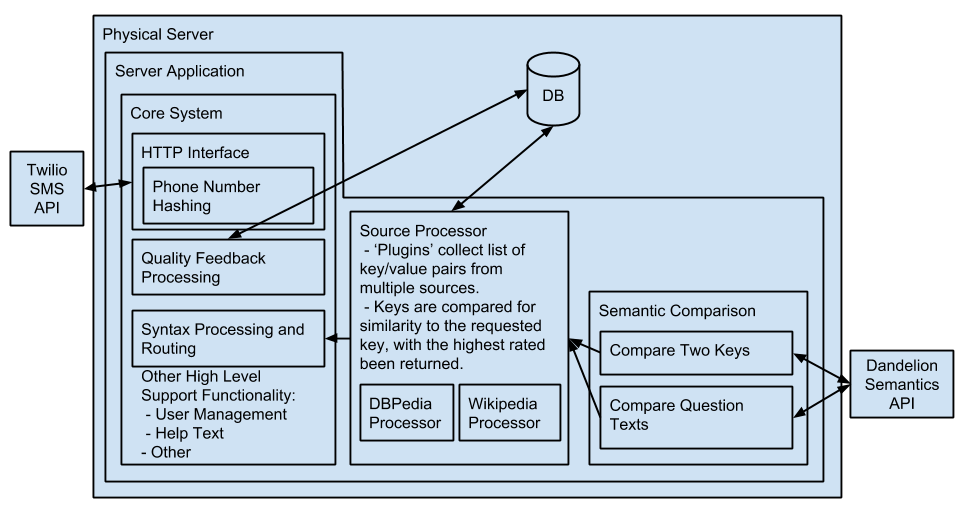
\includegraphics[width=\linewidth]{systemArchitecture}
\caption{System Architecture}
\label{fig:systemArchitecture}
\end{figure}

\subsubsection{Micro-system for Protecting User Identity}

In section \ref{subsubsec:userPrivacyAndDataProtection}, the need to protect the privacy of a user and the general technique that will be used (involving irreversible hashing) are described.  The design of this system will now be discussed.

The main gateway into the system will be an HTTP call to a Python function, which takes the phone number of the user and the question being asked as its parameters.  This function represents a core part of the privacy protection system, by generating the hashed phone number and only using that when calling functions that compute an answer.  The user's phone number is only subsequently used when 

\marginnote{delete this code and finish above sentence}
%todo delete this code and finish above sentence

\begin{lstlisting}[language=Python]
def entry(userCell, question):
    hashedCell = someHashFunction(userCell)
    answer = findAnswer(hashedCell, question)
    return userCell, answer
\end{lstlisting}

The userCell is required at the output of the function to determine the number to which a response will be sent.  However, as the computation of an answer only requires a general constant representation of user identity, not necessarily the user's phone number, the specific value of userCell is not required within the computation of the answer.  As such, a hash is passed into the answer-computing function.  This hash will be used within the database to store a user's history and profile.  This means that only a user's history can be identified from the database, not the actual identity of a user.

\subsection{Language, Platform and Tools and Libraries}
\subsubsection{Language}
\label{section:designLanguage}
The language Python has been selected to be the main language in project for four reasons:
\begin{enumerate}
  \item Python is universally compatible and simple to execute.  Once the server application is written, it will be simple to migrate it between machines and adjust the application's configuration or environment.
  \item Python is commonly used and has significant community support \marginnote{just cite a big community website} in the form of libraries for all the tools that will be used in this project, for example libraries for querying common databases and for sending text messages.  This is useful as it will save time implementing common functionality like database calls.
  \item Python is an extremely flexible language in which it is easy to implement applications of this type without syntax issues.  This fulfils the system requirement in section (\ref{subsubsec:systemRequirementsFunctional}, point \ref{requirement:easyToImplement}) that the application is easy and quick to implement.
  \item The author has significant expertise in the language.
\end{enumerate}

A testing utility will also be created to query the application from a personal computer without using SMS.  A simple OS X Cocoa application will be created that queries the HTTP interface with JSON in the expected format and displays an answer.  Objective-C and and Mac OS X were chosen as the language and platform for this as the author has experience with Objective-C and uses a Mac.  There was no requirement for universal compatibility because the application is only for testing and development purposes.

\subsubsection{Platform}
The development platform of the utility will be Linux.  This is for three reasons:
\begin{enumerate}
  \item Linux manages Python and its libraries in a simple way without complex installers with tools like the Python Package Index (a library repository)~\cite{pypi}.
  \item Common libraries that will be used for creating a HTTP server, creating a REST API\marginnote{Lilian: should I explain what this is somewhere?}, making database queries and sending SMSs tend to be written primarily on the Linux platform.
  \item The author has familiarity with Linux and has access to significant Linux infrastructure under a grant from Rackspace.
\end{enumerate}

As previously stated, the interface to the application will be over the SMS platform.

\subsubsection{Database}
There are three tables of data that need to be stored.  These are the tables for: user profiles, to allow the application to handle queries that make use of 'state' with users; the machine learning of question-answer quality; and an initial intelligence that a new deployment of the application starts with.  Both the conceptual data model and the logical database design are now presented.

\myparagraph{Conceptual Data Model}
% TODO --- - write conceptual database model
There are five entities in the conceptual data model for this project.  These are:

\begin{itemize}
  \item {\bf Users:} An entity that represents a user, purely by an identifier based on their phone number.
  \item {\bf Complete User History:} A history of all questions they have asked previously to allow for future expansion of the system, perhaps to implement a recommendations system.
  \item {\bf Last Question Asked by a User:} An object containing the parameters of the last question.  This allows the system to handle stateful queries based upon a previous query.
  \item {\bf Keyword Pairs Quality Learning:} Will contain the property requested by a user, the property returned to that user, and the number of times a matching was ranked as being either one, two, three, four or five stars.
  \item {\bf Initial Intelligence:} \color{red} Undecided.
\end{itemize}

These entities are shown in Figure \ref{fig:conceptualDatabaseDesignDiagram}, which also shows the entity relationships.

\begin{figure}[htb] 
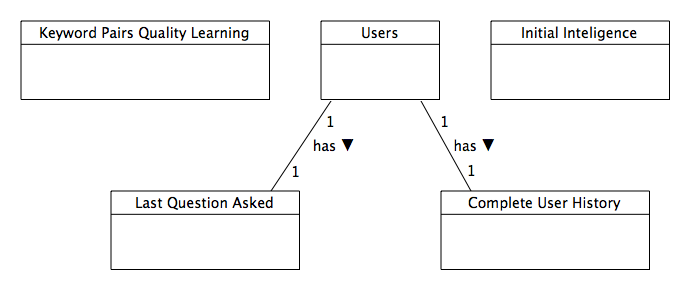
\includegraphics[width=\linewidth]{conceptualModel}
\caption{Conceptual Model of Data}
\label{fig:conceptualDatabaseDesignDiagram}
\end{figure}

\myparagraph{Logical Database Design}
The logical design of the database reduces the number of entities from five in the conceptual model to three.  This is because there is a one-to-one relationship between the \textit{User} entity and both the \textit{Complete User History} and \textit{Last Question Asked by a User} entities, with a small number of fields.  In a large system where relational databases were used it would make sense to keep these entities separate, but in this case merging them allows a wider variety of databases to be used, simplifies the implementation and does not add significantly add to the complexity of the data model. % todo no more 1-1 matching

The logical database requirements are listed in Table \ref{table:logicalDatabaseDesignListing} and represented graphically in Figure \ref{fig:logicalDatabaseDesignDiagram}.

\begin{table}
\begin{center}
    \begin{tabular}{| l | p{6cm} |}
    \hline
    Table/Collection & Parameters \\ \hline
    Users & (\underline{id}, cellNumber, history, lastQuestionText, lastQuestionRequestedProperty, lastQuestionReturnedProperty) \\ \hline
    KeywordRelatednessQuality & (\underline{id}, givenProperty, returnedProperty, oneStarRatings, twoStarRatings, threeStarRatings, fourStarRatings, fiveStarRatings) \\ \hline
    InitialIntelligence & \color{red} Undecided. \\ \hline
    \end{tabular}
    \caption{Logical Database Design.  Underlined fields represent primary keys.}
    \label{table:logicalDatabaseDesignListing}
\end{center}
\end{table}
\marginnote{\color{red}Need to fill in initial intelligence}

\begin{figure}[htb] 
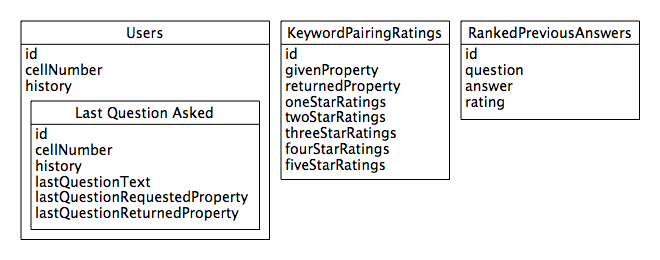
\includegraphics[width=\linewidth]{logicalModel}
\caption{Logical Model of Data}
\label{fig:logicalDatabaseDesignDiagram}
\end{figure}
%todo - remove initial inteligence from the above

\myparagraph{Database Technology}
The database technology requirements for this project are:

\begin{enumerate}
  \item The selected database must be as simple in implementation and interface as possible, whilst still supporting the system requirements.  This is to allow for quick development and to avoid adding unnecessary complexity.
  \item The selected database must allow for storage and retrieval of records with multiple parameters.
  \item Support for records that are related to each other is not required, so relational databases are not needed, but not ruled out.
  \item The database needs to have built-in support for Sharding and Replication/Mirroring to allow the application to scale.
  \item The database must have a library for interfacing with it in the language of this project.
\end{enumerate}

There are a number of database technologies available that would fulfil the data requirements of this project.  These can be split into the categories of relational databases (SQL) and document stores (NoSQL).  Two common database approaches that meet the above requirements are MySQL with an ORM \footnote{ORM: Object-relational mapping tool, which maps queries from the syntax of your programming language to SQL.  ORMs commonly also apply optimisations to queries, and validate them against SQL injections.}, and MongoDB with the Mongo Client.  Table \ref{table:mysqlVsMongo} shows a comparison of both of these technologies.

\begin{table}
\begin{center}
    \begin{tabular}{| p{3.8cm} | p{4.0cm} | p{4.6cm} |}
    \hline
     & MySQL/SQLAlchemy & MongoDB \\ \hline
    Fixed Schema & Yes, reducing flexible & No, giving flexibility \\ \hline
    Querying Simplicity & Requires complex ORM and awareness of transactions, or construction of SQL queries. & MongoDB comes with a Python client, which allows queries in the form of dictionaries. \\ \hline
    Relational Queries Supported & Yes (could be of help in a future extension) & No \\ \hline
    Records support nested parameters & No & Yes \\ \hline
    Built in Sharding support & No & Yes \\ \hline
    Built in Mirroring support & No & Yes \\ \hline
    \end{tabular}
    \caption{MySQL \& SQLAlchemy vs MongoDB}
    \label{table:mysqlVsMongo}
\end{center}
\end{table}

From this comparison, the decision to use MongoDB has been taken because MongoDB has more flexibility than SQL, writing queries is easier in Python and, other than the possibility of future extensions requiring relational structure, it is more scalable than SQL.

\myparagraph{Physical Database Design}
MongoDB separates entities into collections but does not place restrictions on the structure of objects within a collection.  The general structure of the keys in a document (a JSON dictionary) is shown in Table \ref{table:collectionStructure}.

\begin{table}
\begin{center}
    \begin{tabular}{| l | l |}
    \hline
    
    Users &
    \begin{lstlisting}
    {
    '_id',
    'cellNumber',
    'history',
    'lastQuestion' : {
        'text',
        'givenProperty',
        'returnedProperty'
        }
    }
    \end{lstlisting}
    \\ \hline
    
    KeywordRelatednessQuality &
    \begin{lstlisting}
    {
    '_id',
    'givenProperty',
    'returnedProperty',
    'oneStarRatings',
    'twoStarRatings',
    'threeStarRatings',
    'fourStarRatings',
    'fiveStarRatings'
    }
    \end{lstlisting}
    \\ \hline
    
    InitialInteligence &
    \begin{lstlisting}
    Something here
    \end{lstlisting}
    \color{red} Undecided.
    \\ \hline
    
    \end{tabular}
    \caption{Typical Document in each MongoDB Collection}
    \label{table:collectionStructure}
\end{center}
\end{table}

\subsubsection{Libraries}
\myparagraph{Database Querying}
MongoDB comes with a Python client called PyMongo\footnote{For more information: https://api.mongodb.org/python/current/}, which is developed by the same developers as MongoDB.  It is the recommended tool to interact with a MongoDB database~\cite{pyMongoDoc} and has good community support, so it will be used in this project.

\myparagraph{Creating HTTP Server and REST API}
The application needs to have an HTTP interface to allow interactions with it via SMS.  As a result of the non-functional requirement "The system behind the SMS gateway must respond in a timely manner" in section \ref{subsubsec:systemRequirementsNonFunctional}, the application will need to be able to process multiple HTTP requests concurrently to prevent requests queueing up and responses been significantly delayed.

To create an HTTP Interface, the latest Web Server Gateway Interface (WSGI) specification (version 1.0.1, published as PEP 3333)~\cite{eby2010python} will be followed as it is the industry standard. The WSGI specification describes a general interface between web servers and web applications or frameworks (such as Twilio) in the Python language, thus describing how the web server should be constructed.

In this project, two tools are needed: a WSGI server, and a framework for writing WSGI applications. Flask will be used for the framework as the author has extensive experience using it and it is 100\% compliant with the WSGI standard~\cite{libraryFlask}\footnote{100\% compliant according to the Flask product website.}.
\marginnote{footnote: 100\% compliant - remove? It's a note about bias}

With respect to the WSGI server, many implementations exist such as a simple WSGI server included in Flask~\cite{libraryFlask} called Werkzeug~\cite{libraryWerkzeug}, and the Gevent WSGI server~\cite{libraryGevent}.  Support for multiple concurrent HTTP connections is not a requirement in the WSGI specification, and so some WSGI servers such as the implementation of Werkzeug in Flask do not support this\footnote{Werkzeug does support processing multiple HTTP requests concurrently by specifically enabling threading and increasing the default maximum number of processes from one (as described in the documentation at: http://werkzeug.pocoo.org/docs/0.10/serving/ [accessed: 4th April 2015]). However, the implementation of Werkzeug in Flask has these disabled in the source code because Flask uses thread-local storage (memory that is local to a single thread) and so cannot support concurrent HTTP requests on new threads. This is stated on the Flask website at http://flask.pocoo.org/docs/0.10/design/\#thread-locals [accessed: 4th April 2015].}. Gevent does support concurrent HTTP connections~\cite{geventImplementingServers}\footnote{Gevent using the Greenlet library~\cite{libraryGreenlet}, which provides a notion of micro-threading (coroutines). When a new HTTP request is received, Gevent creates a new Greenlet, thus preventing the main thread been blocked and allowing multiple concurrent HTTP requests. The creation of the Greenlet is described in the preceeding reference(\cite{geventImplementingServers}).} and so will be used in this project.

\marginnote{Work these footnotes into the main text}
% TODO Work these footnotes into the main text

\myparagraph{Sending SMS}
There are a number of SMS providers with HTTP gateways available to choose from, all of which are similar. For this project, the provider must match the following criteria:
\begin{itemize}
  \item Forwards received messages to a REST API to enable easy development.
  \item Supports sending messages via a REST API which also enables easy development.
  \item Has good coverage of countries so that users from many countries can use the service.
  \item Has a 'good' reputation. This is because user privacy is still an issue, since data is unencrypted when been sent over SMS, so the provider should be trustworthy.
\end{itemize}

It is difficult to measure the reputation of a provider accurately, but one possible way of doing this is by looking at the number of significant clients they have.

Two services considered were that matched these criteria.  These were Twilio\footnote{Twilio website: https://www.twilio.com/} and Plivo\footnote{Plivo website: https://www.plivo.com/}. Both use REST APIs for handling incoming messages and for sending responses. Both Twilio and Plivo have comparable coverage as well: Twilio state that they send and receive SMS with numbers in 198 countries~\cite{twilioCoverage}, and Plivo state that they support 207 countries~\cite{plivoCoverage}\marginnote{Lilian: remove footnotes about bias?}\footnote{This is referenced on a marketing page (https://www.plivo.com/twilio-alternative/) where Plivo compare their product to Twilio's, so is likely to be biased}. The difference is trivial, as the number of recognised independent states in the world is between 190 and 200 depending on listing; the US Government recognises 195~\cite{usStateDepartmentListOfIndependentStates}.

With regard to reputation, for this project it was decided that Twilio is preferable to Plivo. Although it is difficult to measure reputation accurately, Twilio was founded in 2007 and has an group of clients including PayPal, Uber, Sprint and Airbnb, compared to Plivo, which was founded in 2011 and mainly works with entertainment companies.

\marginnote{citations }
% TODO - citations above

\myparagraph{Semantic Analysis - Measuring semantic relatedness between texts}
\label{sec:choosingSemanticAnalysisApi}
Semantic comparison of text will be used for two purposes within the project: to match keywords from datasources, for example, if a user asks \texttt{how tall} something is, the property \texttt{height} would be appropriate to return; and to match questions with identical meaning to each other to save the application doing a full analysis of the data sources again. The requirements for these use-cases are different: for the former the tool needs to compare pairs of either single words of short strings or words for semantic similiarity; and for the latter the tool needs to be able to compare full sentences for semantic similarity.

Semantic similarity is a measure of how semantically alike entities are in their meaning, for example, \texttt{bank} and \texttt{trust company}~\cite{Budanitsky:2006:EWM:1168106.1168108}. A more general measure exists called Semantic Relatedness. Whereas semantic similarity compares entities by their meaning, entities may be semantically related by additional lexical relationships such as antonymy (the opposite of an entity, for example, \texttt{tall} and \texttt{short}) and meronymy (entities that are a part of another entity, for example, \texttt{car} and \texttt{wheel})~\cite{Budanitsky:2006:EWM:1168106.1168108, budanitsky2001semantic}. Both use-cases in this application will be using semantic similarity as semantic relatedness is too general. An example using the datasource keyword matching usecase is that using semantic relatedness, the word \texttt{tall} would be related to \texttt{width} as well as the target word of \texttt{height} as a result of antonymy, potentially cluttering results. In the second use-case, consider a highly rated question in the database of \texttt{What is the population of England?} and then the question of \texttt{What is the population of London?} being processed. London is a part of England, so there is the potential for the population of England to be returned instead of the population of London.

A key requirement for the algorithm and method used to compute semantic similarity is that it can be implemented in compliance with the system requirement in section \ref{subsubsec:systemRequirementsFunctional}, point \ref{requirement:easyToImplement}, that the system is easy to implement. A number of algorithms were discovered for calculating semantic similarity based on the WordNet lexical database~\cite{wordNet}, such as the Leacock--–Chodorow and Resnik algorithms. Although mathematical representations of these algorithms are published~\cite{leacock1998combining,resnik1995using}, to fulfil the aforementioned requirement a pre-implemented semantic comparison tool is needed as implementation of these algorithms would be a non-trivial software engineering project. Both of the Leacock--–Chodorow and Resnik algorithms are available in a Perl package as part of WordNet::Similarity, a set of Perl modules with an optional web interface for integration into applications. No other open-source libraries were found, so during application design, an attempt was made to use the WordNet::Similarity tools by calling the Perl scripts from Python code. This proved complex as there were numerous out of date dependencies to trace and install.

An alternative to using a specific algorithm in a library was to use an online semantics package. Two were identified: the Cortical Compare API~\cite{serviceCorticalSim}; and the Dandelion Similarity API~\cite{serviceDandelionSim}. Both take two pieces of text and return a value representing the semantic similarity of the texts. The Cortical API was found to be better suited for comparing single word or short multi-word terms using its \texttt{term} type~\cite{serviceCorticalSim}, often returning errors when queried with two texts with a similar syntax, and in contrast the Dandelion API is better suited to single or multi-sentence blocks of text~\cite{dandelionSim}.

Both the Cortical and Dandelion APIs interface via a HTTP REST interface, so will be simple to implement. They are also in active development with support teams. For these reasons, they have been selected to be the semantic comparison tools used in this project.

\myparagraph{Semantic Analysis - Discovering Named Entities in text}
\label{sec:choosingNamedEntityExtractionApi}

A named entity extraction tool is required to establish the geographical entity ('place') in a users' question. The requirements of the tool were:
\begin{enumerate}
  \item Accepts a string of text and returns a list of keywords representing the place.
  \item \label{nexRequirement:categoriseKeyword} Keywords are categorised by a group classes, allowing for differentiation between a keyword representing a place, concept or person.
  \item Accessible via a HTTP REST API for ease of implementation (fulfilling functional system requirement \ref{requirement:easyToImplement} in section \ref{subsubsec:systemRequirementsFunctional}).
\end{enumerate}

During initial research, two keyword extraction APIs were discovered: the Cortical Keyword Extraction API~\cite{serviceCorticalNex} and the Dandelion Named Entity Extraction API~\cite{serviceDandelionNex}. However, the Cortical API does not fulfill requirement \ref{nexRequirement:categoriseKeyword}, simply returning a list of keywords. In comparison the Dandelion API returns a complex data structure which includes a list of DBPedia classes that the keyword is an instance of.

Research was done to identify a way of using the Cortical API to extract keywords and subsequently categorise the keywords after they have been been identified; however as there was no significant benefit of the Cortical API over the Dandelion API this was discounted and the Dandelion API chosen.

Results from the Dandelion API were checked against the \texttt{Place} class in the DBPedia Ontology by checking their \texttt{types} list (a list of DBPedia classes that the keyword fits into) for the string \texttt{http://dbpedia.org/ontology/Place}.

\newpage
\section{Implementation}
\label{sec:implementation}
{\bf This section will contain information on how data is stored, the structure of databases, and the format of and method through which data is sent to an SMS provider.}

Code used within this project is located in the following Git repositories:
\begin{itemize}
  \item \texttt{https://github.com/samheather/dissertationServer} - This repository contains the code for the server application.
  \item \texttt{https://github.com/samheather/dissertationClient} - This repository contains the Xcode Project and code for the Mac OS X testing client, used in development of the application.
  \item \texttt{https://github.com/samheather/dissertationIos} - This repository contains the Xcode Project and code for the iOS client application, used in the experimental evaluation of the application. It has been constructed for an iPhone 5 screen size.
\end{itemize}

\subsection{Implementation Overview}
As discussed in section \ref{sec:method}, the implementation was completed whilst following the iterative development process. Software development took places in stages which represented each iteration, and after each iteration a version of the software was demonstrated in a weekly meeting. In these meetings, the software's capabilities and success rate were discussed, and requirements were re-evaluated based on progress. Ideas for expansions to the software (for example, the Natural Language Processing, which was not in the original plan) were also discussed.

The software has been constructed in a modular manner to allow easy future expansion and modification.

\subsection{Tools and services used}
The following tools and services were used in the implementation. These were chosen to fulfil the requirements detailed in section \ref{sec:method}.
\begin{itemize}
  \item Python was the programming language used in this project. This was due to a number of reasons, including that the author had experience with writing an application with some similar characteristics as those in this project.
  \item MongoDB version 2.6.6 was used as the database software in this project.
  \item Both the application server and the database server were hosted on an Ubuntu version 14.10 "2 GB General Purpose v1" Linux server, hosted by Rackspace in London.
  \item No integrated development environment (IDE) was used in the development of the server application. The author chose to use textural editors due to familiarity with them, and it was felt that the assistance provided by an IDE with managing modularity/abstraction/semantic checking would not be of significant benefit, bearing in mind the size of the server application.
  \item An IDE was used in the development of the client application to reduce the use of expensive SMS during testing. This was written in Objective-C for Mac, and created in the Xcode IDE, which is the industry standard.
  \item The Twilio SMS Service~\cite{serviceTwilio} was used to facilitate the SMS interface to the server application.
  \item The Cortical~\cite{serviceCorticalSim} and Dandelion~\cite{serviceDandelionSim, serviceDandelionNex} APIs were used for semantic analysis of text.
\end{itemize}

In addition, the following Python libraries from the Python Package Index\footnote{Python Package Index website: https://pypi.python.org/pypi} were used within the server application:
\begin{enumerate}
    \item Greenlet~\cite{libraryGreenlet} - provides a notion of micro-threading (coroutines), which allows the server to process multiple HTTP requests concurrently.
    \item gevent~\cite{libraryGevent} \label{librariesUsed:gevent} - a coroutine based networking library for Python. gevent provides a Web Server Gateway Interface (WSGI) server that supports processing multiple requests concurrently, using Greenlet.
    \item PyMongo~\cite{libraryPyMongo} - Python library containing tools to work with MongoDB databases.
    \item ujson~\cite{libraryUjson} - Twilio uses JSON as the format for HTTP requests, so it makes sense to use it for all requests. ujson allows for effecient encoding and decoding of json to and from Python data structures.
    \item Twilio~\cite{libraryTwilio} - Twilio library used for receiving and sending SMS.
    \item lxml~\cite{libraryLxml} - Used in the 'Wikipedia Utils' library, which handles interactions with the Wikipedia API. lxml is used for processing XML/HTML in Python.
    \item Flask~\cite{libraryFlask} - a micro-framework for web applications, used for its simple syntax for defining HTTP routes (URLs that trigger Python functions). Flask also comes with a WSGI server, but it does not support processing multiple HTTP requests concurrently, so it is replaced with the Gevent WSGI server in point \ref{librariesUsed:gevent}.
    \item NumPy~\cite{libraryNumPy} - Numerical Python (NumPy) is used for outlier detection in the rating system. It provides a function call for calculating the standard deviation of a set of numbers.
    \item re - a Regular Expression matching library built into Python which is used in the 'Wikipedia Utils' library and in application code for converting CamelCase text to Snake case text.
    \item Wikipedia Utils~\cite{libraryWikipediaUtils} - a library used for abstracting the Wikipedia API.
\end{enumerate}


\subsection{Implementation of natural language processing module}
In this section, a description of how the natural language processing module was implemented is given.

It was decided that a module should be constructed specifically for the parsing of natural language questions in the application.  This module, called nlp, processes question in natural language form, and is able to output the two parameters needed by the application for answering a question.

The first step in the process is to remove punctuation from the question text, which is of no meaning in the context of this application. Consider an example sentence \texttt{How tall is the Eiffel Tower?}. In this sentence, the question mark will be removed to give \texttt{How tall is the Eiffel Tower}.

\begin{sloppypar} % stops the long url going into the margin
The next step in the process is to identify the geographical entity that a user is investigating. This is done by passing the original question into a Named Keyword Extraction tool, which extracts a list of keywords representing entities from a string and and returns them. The Dandelion Named Entity Extraction tool was selected as in addition to providing a list of words representing entities, it categorised them according to the DBPedia Ontology. By using this, it was possible to identify the geographical entity by simply checking each keyword for the type \texttt{http://dbpedia.org/ontology/Place} in the types associated with each keyword.  This is done by the \texttt{extractEntities()} function in the nlp module.
\end{sloppypar}

The final step in the process is to identify the property that a user is requesting about the entity, for example, the height. This is done in the \texttt{stripToProperty()} function in the nlp module. This function identifies the property by assuming it will be the only text in the sentence with meaning, excluding the place name. As such, the first action of this function is to remove words relating to the name of the geographical entity being queried, which it does by checking each word in the question text against each word in the place string, and removing the word if they are equal. After this process, our example question will have been changed from \texttt{How tall is the Eiffel Tower} to \texttt{How tall is the?}. The next step is to remove meaningless words that do not identify the property that the user querying. These are stop words, such as \texttt{and, the, of}. As with removing words relating to the geographical entity, this is done by checking each word in the question text against a list of stop words and removing them if they match. In our above example, the question text will now be \texttt{tall}. This is the property determined to be the subject of a users' query.

Having called both \texttt{extractEntities()} and \texttt{stripToProperty()}, the nlp module packages these results into a dictionary and returns them as the processed representation of the question text.

\subsection{Implementation of answer location system}
In this section, a description of the process followed to answer a question about a property of a geographical entity is presented. 

After having identified the place and the property of that place in the question using the nlp module, the application must locate the value of that property for that place. This is done in the \texttt{sourceProcessor} module, which collates data from the data sources and then attempts to identify from those sources an answer to the users question.

The entry point into \texttt{sourceProcessor} is the \texttt{findArgumentOnPage()} function, which takes the place name and the property being queried as input parameters. The first step of \texttt{findArgumentOnPage()} is to query the data sources for a dictionary of properties about the geographical entity, pulling down all information available on the entity in question. Interfaces to data sources are factored out into modules, such as \texttt{dbpediaParser} and \texttt{wikiPageParser}, which handle queries to these data sources and return the data to the application in a normalised form (a dictionary of keys and values about the geographical entity).

After having retrieved a list of properties about the entity, the application then iterates through the datasets (one dataset per source) checking the keys against the key in the question text. If any key in the keys for a dataset is an exact, case-insensitive match, the value for that key is returned as the answer. Otherwise, each key in the compared to the requested key for semantic relatedness. This tries to match key strings given in different contexts, and is useful in the case that a user asks a question using a different word to represent the property they require than the one in the data source. After having compared each key to the property given by the user, the key with the highest semantic similarity is returned. 

An example of where the semantic comparison and matching of keys is useful is the question \texttt{How tall is the Eiffel tower?}, where the property string is \texttt{tall}, and in the data source the key might appear as \texttt{height}. The word \texttt{tall} has a high semantic relatedness to the word \texttt{height}, so the value for \texttt{height} will most likely be returned, unless another key with higher semantic similarity is found.

This semantic comparison is done by the the \texttt{compare} module, which has a function \texttt{similarityOfProperty()}. This function takes two strings as an input, and returns a value representing the semantic similarity of the two strings. Two services are used for the semantic comparison: the Cortical~\cite{serviceCorticalSim} and Dandelion~\cite{serviceDandelionSim} similarity APIs.

The Cortical API is not configured for recognising text in CamelCase, so helper functions such as \texttt{camelCaseToSnakeCase} and \texttt{camelCaseToSpace} are also included for converting CamelCase to either Snake Case or space-separated words.

% TODO --- - explain why had to use both, explain why using both is bad
% also talk about issues with compare module, multiple services etc, here
{\bf explain why had to use both, explain why using both is bad}

\subsection{Implementation of rating and learning system}
% TODO XXX - write this

\subsection{Implementation of rating and learning system}
% TODO XXX - write this

\subsection{Discussion of Implementation}
% TODO XXX - write this
 - Tweaking the constants for best results
 - Excluding wikipedia due to dirty data
 
Key issues:

 - can't handle units
 
 - sometimes wikipedia attaches other garbage
 
 - can't do subjective stuff 'depth of the deepest ocean'
 
 - can't do properties that are stored deep within the ontology.

\newpage
\section{Results}
\label{sec:results}
This section's content...

\newpage
\section{Discussion}
\label{sec:discussion}
This section's content...

\newpage

\newpage
\section{Evaluation}
\label{sec:evaluation}
This section's content...

\newpage

\section{Extending this project}
\label{sec:extending}
{\bf Section not complete} %TODO Write extending project
If the author was able to expand this project, areas for expansion include:
\begin{itemize}
  \item Addressing the issue of literacy
  \item Automating the expansion of the database
  \item Units for metrics.
  \item Make it work with all of wikipedia (all pages with infoboxes anyway)
  \item make it work with all languages
  \item use full on random sparql queries to do magic
  \item nlp assumes property is the only other bit of text with meaning. e.g. thank you would break everything.
\end{itemize}

\newpage

\section{Conclusion}
\label{sec:conclusion}
This section's content...

\newpage

{\bf Melby reference not right, publisher weird - ask Lilian in next session.  Url Commented in TEX here} 
%http://scholar.google.co.uk/scholar?hl=en&q=melby+why+cant+a+computer+translate+like+a+person&btnG=&as_sdt=1%2C5&as_sdtp=
\bibliographystyle{IEEEtran}
\bibliography{IEEEabrv,mybib}

\begin{appendices}

\end{appendices}


\newpage
\section{Appendix A - Personas}
\label{sec:appendixPersonas}
\subsection{Nanjala}
%TODO Add photo
\subsubsection{Demographics and Profile}
\begin{itemize}
  \item Female, aged 15
  \item Living in the village of Amuria, Uganda, 300km from the capital Kampala.  Internet access is difficult and expensive to obtain in Amuria, though there is good mobile network coverage.
  \item Currently in general education at her village school.
  \item Nanjala is curious and wants to be able to ask questions and retrieve and read more information at her own leisure.  She prefers to be told about something than to learn facts.
\end{itemize}
\subsubsection{Average Day}
In a typical day, Nanjala will rise early to help her family with housework chores, before she prepares for school.  Nanjala wants to become a teacher.  At school, she studies Science, Maths and Geography, and works hard for her classes and on her homework.  Nanjala's school has a small library and a large body of students, meaning that books are often unavailable when Nanjala would like to look something up.  This increases the amount of time that her homework takes, and can even result in her not having access to information when she goes home.

\newpage
\subsection{Cedric}
%TODO Add photo
\subsubsection{Demographics and Profile}
\begin{itemize}
  \item Male, aged 27
  \item Lives in Zurich, Switzerland, and goes on regular hiking trips, from 3-4 day trips around Europe to longer trips to the South American Andes and southern Asia.
  \item Works in a service role in the city and so has little disposable income to spend on guide books for the many places he visits.
  \item Cedric is a competent albeit not professional hiker, often going off-track and summiting 'difficult' peaks or reaching famous camping grounds.  He likes to be spontaneous, only deciding which peaks he will attempt when he arrives.
  \item Cedric is very conscientious and wants to contribute his own knowledge to the world, especially to projects that help him.
  \item Cedric values his privacy is concerned about how much information he gives out online.
\end{itemize}
\subsubsection{Average European Trip}
A typical trip will involve an intercity train from the Zurich Hauptbahnhof (the main station) to the city closest to the range Cedric will be hiking.  He takes the train because it tends to be cheaper than flights.  Once in the area, Cedric will take local trains and buses to get into the mountain ranges.  There, he will use the local hiking trail network signs and conversations with the locals to select a peak or route.  Once Cedric has got moving and is reaching higher ground, he uses a combination of his view and the signage to identify other peaks that he would like to wander around.  

Cedric takes a non-smart phone with him because a) the battery life on his smart phone is not long enough for his whole trip, whereas his non-smart phone lasts a week at a time, and b) his smart phone would not be useful anyway, since the internet is so intermittent.  He still wishes he could get information such as whether there are maintained routes on the slopes of a given peak or the height of a peak that he sees without having to phone friends back in the city.
\newpage

\section*{Appendix B - Sample Consent Form}
\label{sec:appendixConsentForm}
\newpage

\subsection*{System to access knowledge using Machine Learning and SMS - Usability and Usefulness Study}
{\parindent0pt
\subsubsection*{Informed Consent - Introduction}
This study aims to investigate the usability and usefulness of a system developed to provide access to knowledge using machine learning and SMS.  The system aims to provide high quality answers to questions asked of it, where the questions relate to either a description or property of a geographical entity (for example a city, river or mountain).  The system aims to learn where mistakes have been made and improve by receiving feedback from the user on the previous answer.  

\subsubsection*{Form: please complete this section before the study.}
I, \textunderscore\textunderscore\textunderscore\textunderscore\textunderscore\textunderscore\textunderscore\textunderscore\textunderscore\textunderscore\textunderscore\textunderscore\textunderscore\textunderscore\textunderscore\textunderscore\textunderscore\textunderscore\textunderscore\textunderscore\textunderscore\textunderscore\textunderscore\textunderscore\textunderscore\textunderscore\textunderscore\textunderscore\textunderscore\textunderscore\textunderscore\textunderscore\textunderscore\textunderscore\textunderscore\textunderscore\textunderscore\textunderscore\textunderscore\textunderscore\textunderscore\textunderscore, agree to participate in this study.  I have been briefed on and understand the purpose and goals of the project.

I understand that information will be collected from me during this study in the form of my answers to a questionnaire.  Additionally, I understand that my interactions with the application will be recorded, specifically the questions I ask, answers returned and my quality ratings of answer. I understand that this information will be treated confidentially and only Sam Heather and the project supervisor (Lilian Blot) will have access to the original data in its original format.  When the information is processed, shared, described or interpreted I will not be personally identified.

I understand that I can withdraw from the study at any point without giving a reason.

Date: \textunderscore\textunderscore\textunderscore\textunderscore\textunderscore\textunderscore\textunderscore\textunderscore\textunderscore\textunderscore\textunderscore\textunderscore\textunderscore\textunderscore\textunderscore\textunderscore\textunderscore\textunderscore\textunderscore\textunderscore\textunderscore
Signature: \textunderscore\textunderscore\textunderscore\textunderscore\textunderscore\textunderscore\textunderscore\textunderscore\textunderscore\textunderscore\textunderscore\textunderscore\textunderscore\textunderscore\textunderscore\textunderscore\textunderscore\textunderscore\textunderscore\textunderscore\textunderscore

{\bf Researcher's contact details:} Sam Heather, sam@heather.sh

{\bf Supervisor's contact details:} Lilian Blot, lilian.blot@york.ac.uk

\pagebreak

\subsubsection*{Post experiment consent form - please complete this section after the study.}
$\square$ I have been suitably debriefed about the system and my performance.

$\square$ I understand I can withdraw my data from the study at any time.

$\square$ I have not been forced to take part in this study.

$\square$ The Researcher has treated me with respect and answered all of my questions.

\vspace{10 mm}

For the researcher: Participant ID: \textunderscore\textunderscore\textunderscore\textunderscore\textunderscore

}

\newpage
\section{Appendix C - Sample Questionnaire}
\label{sec:appendixQuestionnaire}
\newpage

\subsection*{Please fill in the following questionnaire with regard to your experience of the system that has been developed.}.

\begin{tabular}{|m{0.5cm}|m{7.0cm}|>{\centering\arraybackslash}m{4cm}|}
\hline
\centering \# &
\centering Question &   
\centering Agreement \\ 1 = strongly disagree \\ 3 = neutral \\ 5 = strongly agree \tabularnewline
\hline
1  & 
Using the system would enable me to locate information more quickly when without access to the internet  & 
1 \ 2 \ 3 \ 4 \ 5
\tabularnewline
\hline
2  & 
Using the system would improve my performance when working or researching without access to the internet  & 
1 \ 2 \ 3 \ 4 \ 5
\tabularnewline
\hline
3  & 
Using the system would increase my productivity when performing casual research without access to the internet  & 
1 \ 2 \ 3 \ 4 \ 5
\tabularnewline
\hline
4  & 
Using the system would enhance my effectiveness at finding information without the internet  & 
1 \ 2 \ 3 \ 4 \ 5
\tabularnewline
\hline
5  & 
Using the system would make it easier for me to find information without access to the internet  & 
1 \ 2 \ 3 \ 4 \ 5
\tabularnewline
\hline
6  & 
I would find the system useful in day-to-day life when without access to the internet  & 
1 \ 2 \ 3 \ 4 \ 5
\tabularnewline
\hline
7  & 
Learning to operate the system was easy for me  & 
1 \ 2 \ 3 \ 4 \ 5
\tabularnewline
\hline
8  & 
I would find it easy to get the system to do what I want it to do  & 
1 \ 2 \ 3 \ 4 \ 5
\tabularnewline
\hline
9  & 
My interaction with the system would be clear and understandable  & 
1 \ 2 \ 3 \ 4 \ 5
\tabularnewline
\hline
10  & 
I found the system to be flexible to interact with  & 
1 \ 2 \ 3 \ 4 \ 5
\tabularnewline
\hline
11  & 
It would be easy for me to become skilful at using the system  & 
1 \ 2 \ 3 \ 4 \ 5
\tabularnewline
\hline
12  & 
I found the system easy to use & 
1 \ 2 \ 3 \ 4 \ 5
\tabularnewline
\hline
13  & 
The information returned was useful, relevant, and answered the question asked & 
1 \ 2 \ 3 \ 4 \ 5
\tabularnewline
\hline
14  & 
I trust the answers returned by this application & 
1 \ 2 \ 3 \ 4 \ 5
\tabularnewline
\hline
\end{tabular}

\vspace{10 mm}

For the researcher: Participant ID: \textunderscore\textunderscore\textunderscore\textunderscore\textunderscore



\end{document}  %End of document.



















